\documentclass[11pt,letterpaper]{article}
\usepackage[utf8]{inputenc}
\usepackage[left=1in,right=1in,top=1in,bottom=1in]{geometry}
\usepackage{amsfonts,amsmath}
\usepackage{graphicx,float}
% -----------------------------------
\usepackage{hyperref}
\hypersetup{%
  colorlinks=true,
  linkcolor=blue,
  citecolor=blue,
  urlcolor=blue,
  linkbordercolor={0 0 1}
}
% -----------------------------------
\usepackage[style=authoryear-icomp,backend=biber]{biblatex}
\addbibresource{citation.bib}
% -----------------------------------
\usepackage{fancyhdr}
\newcommand\course{MATH-UA.0252\\Numerical Analysis}
\newcommand\hwnumber{12}                  % <-- homework number
\newcommand\NetIDa{Ryan Sh\`iji\'e D\`u} 
\newcommand\NetIDb{December 8th, 2023}
\pagestyle{fancyplain}
\headheight 35pt
\lhead{\NetIDa\\\NetIDb}
\chead{\textbf{\Large Worksheet \hwnumber}}
\rhead{\course}
\lfoot{}
\cfoot{}
\rfoot{\small\thepage}
\headsep 1.5em
% -----------------------------------
\usepackage{titlesec}
\renewcommand\thesubsection{(\arabic{section}.\alph{subsection})}
\titleformat{\subsection}[runin]
        {\normalfont\bfseries}
        {\thesubsection}% the label and number
        {0.5em}% space between label/number and subsection title
        {}% formatting commands applied just to subsection title
        []% punctuation or other commands following subsection title
% -----------------------------------
\setlength{\parindent}{0.0in}
\setlength{\parskip}{0.1in}
% -----------------------------------
\newcommand{\de}{\mathrm{d}}
\newcommand{\DD}{\mathrm{D}}
\newcommand{\pe}{\partial}
\newcommand{\mcal}{\mathcal}
%\newcommand{\pdx}{\left|\frac{\partial}{\partial_x}\right|}

\newcommand{\dsp}{\displaystyle}

\newcommand{\norm}[1]{\left\Vert #1 \right\Vert}
%\newcommand{\mean}[1]{\left\langle #1 \right\rangle}
\newcommand{\mean}[1]{\overline{#1}}
\newcommand{\inner}[2]{\left\langle #1,#2\right\rangle}

\newcommand{\ve}[1]{\boldsymbol{#1}}

\newcommand{\thus}{\Rightarrow \quad }
\newcommand{\fff}{\iff\quad}
\newcommand{\qdt}[1]{\quad \mbox{#1} \quad}

\renewcommand{\Re}{\mathrm{Re}}
\renewcommand{\Im}{\mathrm{Im}}
\newcommand{\E}{\mathbb{E}}
\newcommand{\lap} {\nabla^2}
\renewcommand{\div}{\nabla\cdot}

\newcommand{\csch}{\text{csch}}
\newcommand{\sech}{\text{sech}}


\newcommand{\hot}{\text{h.o.t.}}

\newcommand{\ssp}{\left.\qquad\right.}

\newcommand{\var}{\text{var}}
\newcommand{\cov}{\text{cov}}

%%%%%%%%%%%%%%%%%%%%%%%%%%%%%%%%%%%%%%%%%%%%%%%%%%
\makeatletter
\newcommand*{\mint}[1]{%
  % #1: overlay symbol
  \mint@l{#1}{}%
}
\newcommand*{\mint@l}[2]{%
  % #1: overlay symbol
  % #2: limits
  \@ifnextchar\limits{%
    \mint@l{#1}%
  }{%
    \@ifnextchar\nolimits{%
      \mint@l{#1}%
    }{%
      \@ifnextchar\displaylimits{%
        \mint@l{#1}%
      }{%
        \mint@s{#2}{#1}%
      }%
    }%
  }%
}
\newcommand*{\mint@s}[2]{%
  % #1: limits
  % #2: overlay symbol
  \@ifnextchar_{%
    \mint@sub{#1}{#2}%
  }{%
    \@ifnextchar^{%
      \mint@sup{#1}{#2}%
    }{%
      \mint@{#1}{#2}{}{}%
    }%
  }%
}
\def\mint@sub#1#2_#3{%
  \@ifnextchar^{%
    \mint@sub@sup{#1}{#2}{#3}%
  }{%
    \mint@{#1}{#2}{#3}{}%
  }%
}
\def\mint@sup#1#2^#3{%
  \@ifnextchar_{%
    \mint@sup@sub{#1}{#2}{#3}%
  }{%
    \mint@{#1}{#2}{}{#3}%
  }%
}
\def\mint@sub@sup#1#2#3^#4{%
  \mint@{#1}{#2}{#3}{#4}%
}
\def\mint@sup@sub#1#2#3_#4{%
  \mint@{#1}{#2}{#4}{#3}%
}
\newcommand*{\mint@}[4]{%
  % #1: \limits, \nolimits, \displaylimits
  % #2: overlay symbol: -, =, ...
  % #3: subscript
  % #4: superscript
  \mathop{}%
  \mkern-\thinmuskip
  \mathchoice{%
    \mint@@{#1}{#2}{#3}{#4}%
        \displaystyle\textstyle\scriptstyle
  }{%
    \mint@@{#1}{#2}{#3}{#4}%
        \textstyle\scriptstyle\scriptstyle
  }{%
    \mint@@{#1}{#2}{#3}{#4}%
        \scriptstyle\scriptscriptstyle\scriptscriptstyle
  }{%
    \mint@@{#1}{#2}{#3}{#4}%
        \scriptscriptstyle\scriptscriptstyle\scriptscriptstyle
  }%
  \mkern-\thinmuskip
  \int#1%
  \ifx\\#3\\\else_{#3}\fi
  \ifx\\#4\\\else^{#4}\fi  
}
\newcommand*{\mint@@}[7]{%
  % #1: limits
  % #2: overlay symbol
  % #3: subscript
  % #4: superscript
  % #5: math style
  % #6: math style for overlay symbol
  % #7: math style for subscript/superscript
  \begingroup
    \sbox0{$#5\int\m@th$}%
    \sbox2{$#5\int_{}\m@th$}%
    \dimen2=\wd0 %
    % => \dimen2 = width of \int
    \let\mint@limits=#1\relax
    \ifx\mint@limits\relax
      \sbox4{$#5\int_{\kern1sp}^{\kern1sp}\m@th$}%
      \ifdim\wd4>\wd2 %
        \let\mint@limits=\nolimits
      \else
        \let\mint@limits=\limits
      \fi
    \fi
    \ifx\mint@limits\displaylimits
      \ifx#5\displaystyle
        \let\mint@limits=\limits
      \fi
    \fi
    \ifx\mint@limits\limits
      \sbox0{$#7#3\m@th$}%
      \sbox2{$#7#4\m@th$}%
      \ifdim\wd0>\dimen2 %
        \dimen2=\wd0 %
      \fi
      \ifdim\wd2>\dimen2 %
        \dimen2=\wd2 %
      \fi
    \fi
    \rlap{%
      $#5%
        \vcenter{%
          \hbox to\dimen2{%
            \hss
            $#6{#2}\m@th$%
            \hss
          }%
        }%
      $%
    }%
  \endgroup
}

\begin{document} 

\section{Inner product}
\subsection{}
Let's define a new inner product in $\mathbb R^3$ with a symmetric
  positive-definite matrix $W\in \mathbb R^{3\times 3}$ as follows:
  $$
  \langle \boldsymbol u, \boldsymbol v\rangle_W := \boldsymbol u^\top W \boldsymbol v
  $$
  Show that this defines an inner product on $\mathbb R^3$ and write
  down the induced norm. If 
  $$W=\begin{bmatrix}2& -1& 0 \\ -1 & 2 & -1
  \\ 0 & -1 & 2 \end{bmatrix},$$
  give a vector that is orthogonal to
  $[1,0,0]^\top$ in the $W$-inner product.

\subsection{}
Now let's consider a symmetric positive
  semi-definite matrix. Does the above definition still define an
  inner product and why/why not?


\section{Orthogonal polynomial with weight}
We assume
  an inner product on $[-1,1]$ with weight $\omega(x):=1-x^2$, i.e.,
  $$
  \langle p,q\rangle = \int_{-1}^1 \omega(x)p(x)q(x)\,\de x.
  $$ We define the following polynomials, which are orthogonal with
  respect to this inner product:
  $$
  \varphi_0(x) = 1, \quad \varphi_1(x) = 2x, \quad \varphi_2(x) = 5x^2-1
  $$

\subsection{}
Verify that $\varphi_0$ and $\varphi_1$ are orthogonal on $[-1,1]$
    with respect to the weight $\omega$.

\subsection{}
Are the $\varphi_j$'s orthonormal under this inner product?

\subsection{}
Find the polynomial $p \in \boldsymbol P_2$ for which
    $\displaystyle \int_{-1}^1 (1-x^2)(p(x) - x^3)^2 \, \de x$ is minimal.


\section{Best 2-norm approximation}
\subsection{} 
The upper row in the below figure shows a function $f$ together with a polynomial approximation. For three plots, the
      optimal best 2-norm fit for three different weights $w(x)$ is
      used, and one is the result of an Lagrange interpolation. Match
      the approximations in the upper row with the information (weight
      functions or interpolation points) in the lower row.
      \begin{center}
        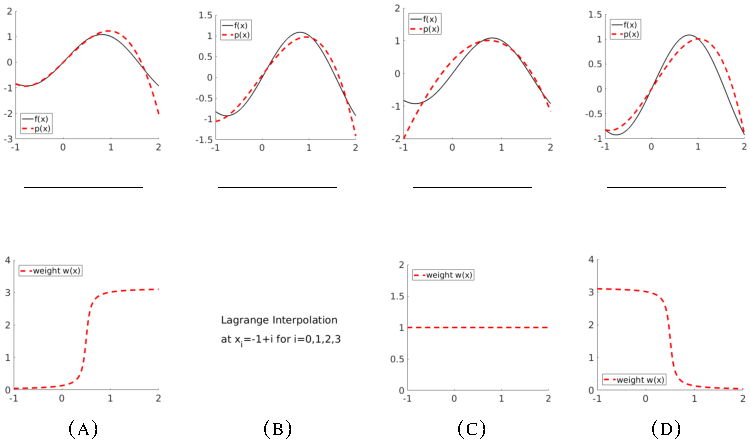
\includegraphics[width=.9\textwidth]{bestL2}
      \end{center}
\subsection{} 
Let$\{\varphi_0, \varphi_1, \varphi_2\}$ be a system of
      ortho\textit{normal} polynomials on $[-1,1]$ with respect to the
      weight function $w(x)=\sqrt{1-x^2}$ given by
      \[ \varphi_0(x)=\sqrt{\frac{2}{\pi}},\quad
      \varphi_1(x)=2x\sqrt{\frac{2}{\pi}}, \quad
      \varphi_2(x)=(4x^2-1)\sqrt{\frac{2}{\pi}}.
      \]
      Given $f(x)=\frac{2}{\sqrt{1-x^2}}$, find the polynomial best fit of
      degree 2 in the weighted 2-norm.



\vfill
\printbibliography

\end{document}